\chapter{Resultado das Avaliações}
  
  Essa seção apresenta o resultados das avaliações feitas ao longo do projeto.
  
  \section{Avaliações do protótipo de papel}
     
     Para se realizar a avaliação do protótipo de papel, foi solicitado a 5 usuários com um perfil comum
     e compatível com a proposta do aplicativo (frequentadores de eventos), que realizassem dois cenários para a avaliação:
  
    \begin{itemize}
	\item A - Criar uma notificação com data e hora definidos.
	\item B - Gerenciar (edição e exclusão) suas notificações agendadas.
    \end{itemize}
     
    \noindent
    \textbf{Questionários aplicados}
    
      Foi solicitado que os usuários respondessem, ao final de cada cenário realizado, às três questões do
      questionário ASQ (em anexo).            
  
    \subsection{1ª iteração de avaliação}
        
          A tabela \ref{opnioes1iteracao} descreve o \textit{feedback} dos usuários com os pontos que faltaram na aplicação:
	
  \begin{table}[h]
  \centering
  \begin{tabular}{|m{1.5cm}||m{15cm}|}
    \hline
    \textbf{Usuário} & \textbf{Sentiu falta de:}\\
    
    \hline                               
    1 & 
      \begin{itemize}
	\item Um campo para escolher a cidade do evento na tela de escolher para quando deseja a notificação.
	\item Mensagem de confirmação de exclusão de uma notificação.
      \end{itemize}\\

    \hline                               
    2 & 
      \begin{itemize}
	\item Mensagem de notificação da perda dos dados caso queira voltar para uma tela anterior.
	\item A possibilidade de escolher um intervalo de horário para a notificações, ao invés de um horário fixo.
	\item Ao invés de colocar a mensagem de confirmação do salvamento de uma notificação em uma tela separada, colocar como uma mensagem sobrepondo a mesma tela.
	\item As notificações agendadas poderiam aparecer logo na página inicial.
      \end{itemize}\\
    
    \hline                               
    3 & 
      \begin{itemize}
	\item Uma melhor visualização do campo que exibe as notificações adicionadas.
	\item Lista de notificações agendadas mais centralizada.
	\item Símbolo de “Retirar tema” mais intuitivo.
	\item Caixinha de “Mais temas” na tela de edição.
      \end{itemize}\\
    
    \hline                               
    4 & 
    \begin{itemize}
      \item Especificação que a notificação de horário é referente a notificação.
      \item Melhorar símbolo de “menos” na tela de “Editar notificação”.
    \end{itemize}\\
    
    \hline                               
    5 & 
    \begin{itemize}
      \item Espaço para comentários sobre uma notificação. Ex: Comprar ingresso para a tia Tânia.
    \end{itemize}\\
    
    \hline
  \end{tabular}
  \caption{Opniões dos usuários na 1ª iteração de avaliação.}
  \label{opnioes1iteracao}
  \end{table}
  
  Na figura \ref{resposta_asq_1iteracao} se encontram as respostas ao questionário ASQ pelos cinco usuários avaliados.

  \begin{figure}[!htb]
  \centering
  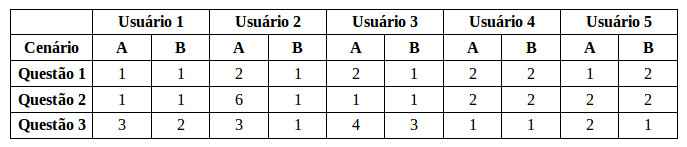
\includegraphics[scale=0.6]{figuras/nota1avaliacao.jpg}
  \caption{Resposta dos usuários ao questionário ASQ na primeira avaliação do protótipo de papel}
  \label{resposta_asq_1iteracao}
  \end{figure}
    
    \pagebreak
    \subsection{2ª iteração de avaliação}
	
	  A tabela \ref{opnioes2iteracao} descreve o \textit{feedback} dos usuários com os pontos que faltaram na aplicação:
	
  \begin{table}[h]
  \centering
  \begin{tabular}{|m{1.5cm}||m{15cm}|}
    \hline
    \textbf{Usuário} & \textbf{Sentiu falta de:}\\
    
    \hline                               
    1 & 
      \begin{itemize}
	\item Deixar as informações na tela mais divididas.
	\item Uma opção ao usuário de registro.
      \end{itemize}\\

    \hline                               
    2 & 
      \begin{itemize}
	\item Cancelar a edição da notificação.
	\item Fazer confirmação de alterado com sucesso.
      \end{itemize}\\
    
    \hline                               
    3 & 
      \begin{itemize}
	\item Programar para aviso prévio (não no dia).
	\item A cidade ser a primeira a ser selecionada para limitação do seventos.
      \end{itemize}\\
    
    \hline                               
    4 & 
    \begin{itemize}
      \item Deixar o "Não" destacado da opção de excluir notificação.
    \end{itemize}\\
    
    \hline                               
    5 & 
    \begin{itemize}
      \item Não há sugestões.
    \end{itemize}\\
    
    \hline
  \end{tabular}
  \caption{Opniões dos usuários na 2ª iteração de avaliação.}
  \label{opnioes2iteracao}
  \end{table}
  
  
  
  Na figura \ref{resposta_asq_2iteracao} se encontram as respostas ao questionário ASQ pelos cinco usuários avaliados.

  
  
  \begin{figure}[!htb]
  \centering
  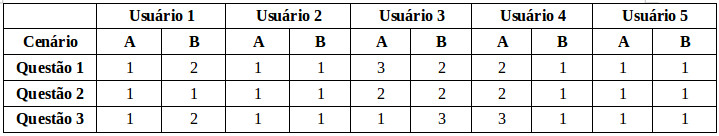
\includegraphics[scale=0.7]{figuras/nota2avaliacao.jpg}
  \caption{Resposta dos usuários ao questionário ASQ na segunda avaliação do protótipo de papel}
  \label{resposta_asq_2iteracao}
  \end{figure}
  
    \pagebreak
  \subsection{Análise dos resultados da avaliação do protótipo de papel}
    
    \subsubsection{1ª iteração}
      
      Na primeira iteração, o objetivo primário de levantar requisitos foi cumprido com louvor.
      Todas as colocações levantadas pelos usuários foram analisadas pela equipe e aceitas quase que totalmente.
            
      Com a aplicação do questionário ASQ, foi possível avaliar a facilidade de uso do aplicativo, a reação do usuário 
      com o tempo gasto para realizar as tarefas e satisfação do usuário com o suporte do aplicativo, mesmo na primeira
      fase de prototipação. Com esses dados é possível perceber a evolução do protótipo em relação à percepção do usuário.
      
    \subsubsection{2ª iteração}
    
      Na segunda iteração poucas colocações foram levantadas pelos usuários avaliados, mas as que foram levantadas também foram
      analisadas pela equipe e consideradas para a construção do protótipo de mais alta fidelidade.
      
      Não foi feita outra iteração de avaliação do protótipo de papel porque nesta iteração surgiram poucas mudanças,
      evidenciando a estabilização do protótipo de papel.
      
      Nessa iteração também foram coletadas as respostas ao questionário ASQ. A análise dos dados se encontra logo abaixo.
    
    \subsubsection{Análise geral}
      
      Apesar do objetivo da avaliação com o protótipo de papel ser o levantamento de possíveis requisitos,
      objetivo que foi alcançado com as iterações que foram realizadas, foi possível levantar alguns pontos
      no quesito de usabilidade, como é possível ver nas tabelas \ref{opnioes1iteracao} e \ref{opnioes2iteracao}.
      As colocações pertinentes referentes à usabilidade do protótipo foram consideradas para a evolução do protótipo.
      
      Com o surgimento de novos requisitos, sugeridos pelos usuários, a equipe viu a necessidade de quebrar o requisito
      "Gerenciar notificações agendadas" em "Alterar notificações agendadas" e "Excluir notificações agendadas", que acabou
      criando mais dois cenários de avaliação para a iteração de avaliação do protótipo de alta fidelidade (descritos
       na próxima seção).
      
      O registro das respostas dos usuários ao questionário ASQ permitiu ver a evolução dos cenários nas versões do 
      protótipo de papel. Foi tirada a média das respostas dos cinco usuários avaliados para cada iteração de avaliação
      e o resultado se encontra na figura \ref{evolucao_prototipo_papel_ASQ}.
      
      \begin{figure}[!htpb]
	\centering
	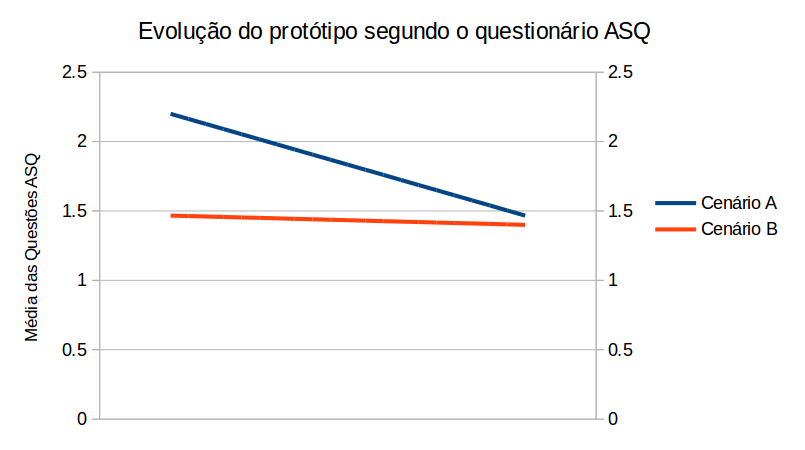
\includegraphics[scale=0.35]{editaveis/figuras/evolucao_prototipo_papel_ASQ}
	\caption[Evolução do protótipo de papel, segundo o questionário ASQ]
	  {Evolução do protótipo de papel, segundo o questionário ASQ.}
	\label{evolucao_prototipo_papel_ASQ}
      \end{figure}
      
      Pelo gráfico apresentado na figura \ref{evolucao_prototipo_papel_ASQ}, é possível ver que houve uma evolução significativa
      no protótipo no cenário A, enquanto no cenário B houveram poucas mudanças. No geral, percebe-se que o protótipo evoluiu
      bem na percepção dos usuários, uma vez que, segundo a pontuação proposta pelo ASQ, quanto mais próximo de 1 estiver
      a pontuação das respostas às perguntas, mais o usuário concorda e está satisfeito com o cenário.
  
  \vfill
  \pagebreak
  \section{Avaliações do protótipo de alta fidelidade}
    
      Para se realizar a avaliação do protótipo de alta fidelidade, foi solicitado a 5 usuários com um perfil comum
      e compatível com a proposta do aplicativo (frequentadores de eventos), que realizassem tarefas em 
      três cenários para a avaliação:
    
      \begin{itemize}
	  \item Cenário A - Criar uma nova notificação para determinado tema, sem adicionar um comentário.
	  \item Cenário B - Editar a hora da notificação criada e adicionar um comentário à notificação.
	  \item Cenário C - Apagar a notificação criada.
      \end{itemize}
      
      \noindent
      \textbf{Questionários aplicados}
      
	Foi solicitado que os usuários respondessem, ao final de cada cenário realizado, às três questões do
	questionário ASQ (em anexo). Ao se completar os três cenários propostos era solicitado que os mesmos 
	respondessem às dezenove questões do questionário PSSUQ (em anexo).
    
    \subsection{1ª iteração de avaliação}
      
	        Logo abaixo são apresentados os resultados da primeira iteração de avaliação do protótipo.
      
      \begin{itemize}
       \item \textbf{Descrição e metodologia do roteiro da avaliação}
       
       \subitem O objetivo dessa avaliação é analisar qual a satisfação obtida pelo usuário ao utilizar o protótipo considerando as seguintes 
       metas e princípios de usabilidade, além das heurísticas definidas por Nielsen:
       \begin{itemize}

	\item Utilidade
        \item Eficácia
        \item Eficiência
        \item Visibilidade
        \item Feedback
        
       \end{itemize}
       
       \item \textbf{Comportamento dos usuários}
       
       \subitem Ao todo, os cinco usuários que avaliaram o protótipo conseguiram cumprir todas as tarefas estabelecidas 
       de todos os cenários. Agiram perante as atividades do protótipo de maneira intuitiva, apesar de ficarem 
       desatentos em relação a alguns ícones, e não demoraram a cumprir as funcionalidades dos cenários de avaliação 
       estabelecidos.
       
       \item \textbf{Resumo das entrevistas}
       
       \subitem Alguns usuários estavam com vergonha de realizar a avaliação pelo fato de ter que fazer uma gravação em vídeo. 
       Devido a isso, foi questionado a eles se os mesmos estavam realmente seguros de realizar a avaliação ou se desejavam 
       interromper a mesma e não realizá-la. Nessa primeira iteração, nenhum dos usuários se negaram e decidiram por 
       continuar a avaliação. As avaliações foram realizadas de maneira mais rápida do que as avaliações do protótipo de papel, 
       devido ao fato de o protótipo de alta fidelidade possuir funções que o tempo de resposta se reduz e não possui mais a 
       necessidade de ficar passando folha a folha do protótipo como ocorria nas avaliações do protótipo de papel.
       
       \item \textbf{Problemas de usabilidade identificados}
       
       \subitem No momento da avaliação, através de observações feitas pela equipe e por análise nos vídeos coletados, foram percebidos 
       alguns problemas de usabilidade que os usuários estiveram no momento da interação com o protótipo. Tais como:
       
       \begin{itemize}
       
       \item Dificuldade em entender o significado do horário da notificação.
       
       \item Dificuldade em identificar o ícone para adicionar o tema da notificação.
       
       \item Dificuldade em identificar o ícone para editar uma notificação.
       
       \item Dificuldade em identificar o ícone para excluir uma notificação.
       
       \end{itemize}
       
       \item \textbf{Paradas críticas}
       
       \subitem No momento da avaliação não houve nenhum caso a qual o usuário ficou sem reação em relação à execução de algum cenário. 
       Quando os mesmos obtiveram dificuldades com alguns ícones, estes ícones foram encontrados no momento da execução.
       
       \item \textbf{Plano de correção}
       
       \subitem Para corrigir os problemas de usabilidade que foram identificados para esta iteração, a equipe vai melhoras a interface do 
       protótipo aumentando os botões dos ícones para deixá-los mais visíveis, pois assim ficará mais intuitivo para o usuário qual 
       atividade aquele ícone vai realizar.
       
      \end{itemize}
      
      Na figura \ref{asqalta} se encontram as respostas ao questionário ASQ pelos cinco usuários avaliados.
      
  \begin{figure}[!htb]
  \centering
  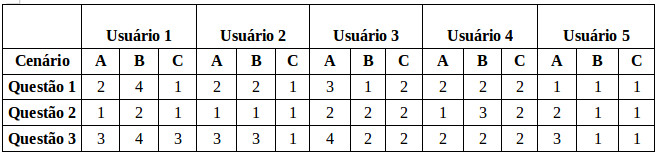
\includegraphics[scale=0.6]{figuras/asqalta.jpg}
  \caption{Resposta dos usuários ao questionário ASQ na primeira avaliação do protótipo de alta fidelidade}
  \label{asqalta}
  \end{figure}
      
      Na figura \ref{pssuqalta} se encontram as respostas ao questionário PSSUQ pelos cinco usuários avaliados.
      
  \begin{figure}[!htb]
  \centering
  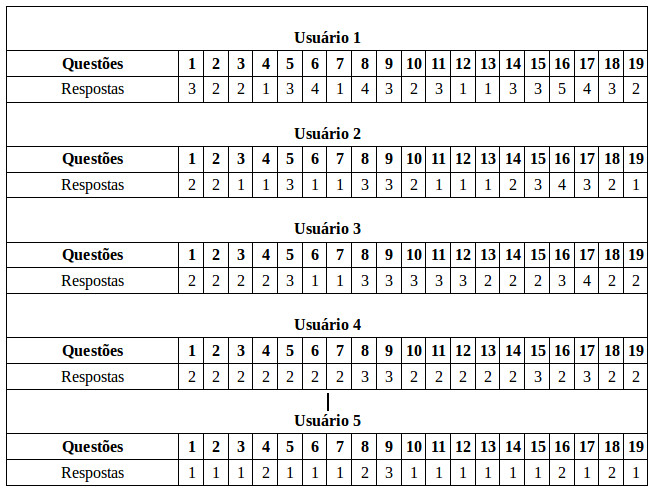
\includegraphics[scale=0.6]{figuras/pssuqalta.jpg}
  \caption{Resposta dos usuários ao questionário PSSUQ na primeira avaliação do protótipo de alta fidelidade}
  \label{pssuqalta}
  \end{figure}
  
      \pagebreak
      
    \subsection{2ª iteração de avaliação}
	
	  Logo abaixo são apresentados os resultados da segunda iteração de avaliação do protótipo de alta fidelidade,
  seguindo o planejamento realizado.
  
  \begin{itemize}
    \item \textbf{Descrição e metodologia do roteiro da avaliação}
    
    \subitem O objetivo da avaliação era analisar qual a satisfação obtida pelo usuário ao utilizar o protótipo, 
    considerando as seguintes metas:
    
    \begin{itemize}
      \item Utilidade;
	\subitem Avaliada pela dimensão \textit{SysUse} do questionário PSSUQ.
	
      \item Eficácia e eficiência;
	\subitem Avaliada pelas dimensões \textit{SysUse} e \textit{InfoQual} do questionário PSSUQ.
	
      \item Interface esteticamente agradável.
	\subitem Avaliada pela dimensão \textit{InterQual} do questionário PSSUQ.
    \end{itemize}
    
    \item \textbf{Comportamento dos usuários}
    
    \subitem Nesta iteração os usuários  agora estavam conseguindo apertar nos botões, pois eles foram aumentados. O que ocorreu é 
    que a funcionalidade de adicionar um tema ainda não estava intuitiva. O botão "+" estava passando despercebido pelos 
    usuários, mesmo este estando maior. Isso fazia com que os usuários não conseguissem prosseguir com a realização da
    funcionalidade de maneira rápida.
    
    
    \item \textbf{Resumo das entrevistas}
    
      \subitem As entrevistas foram realizadas na própria universidade. Estas foram gravadas e cada uma durou em 
	  média 10 minutos contando com o tempo que o usuário teve pra responder os questionários de avaliação.
	  
	  Os usuários deram \textit{feedback} positivo nas entrevistas com as sugestões 
	    
    \item \textbf{Problemas de usabilidade identificados}
    
      \subitem ícone de adicionar o tema da notificação não estava tão intuitivo para o usuário.
          
    \item \textbf{Paradas críticas}
    
      \subitem Não houveram paradas críticas nas avaliações realizadas.
    
    \item \textbf{Plano de correção}
    
      \subitem Para a terceira versão do protótipo, ao invés de apenas um botão de adicionar o tema da notificação, 
      agora cada tema terá em sua frente um ícone. Desta maneira, a equipe de avaliadores acredita que os usuários 
      conseguirão entender de maneira mais rápida como que se adiciona um tema.
    
  \end{itemize}
  
  Na figura \ref{asqalta_2} se encontram as respostas ao questionário ASQ pelos cinco usuários avaliados.
  
  Na figura \ref{pssuqalta_2} se encontram as respostas ao questionário PSSUQ pelos cinco usuários avaliados.
  
  \begin{figure}[!htb]
  \centering
  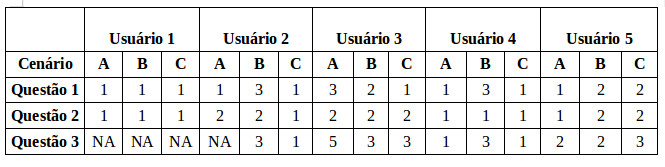
\includegraphics[scale=0.6]{figuras/asqalta_2.jpg}
  \caption{Resposta dos usuários ao questionário ASQ na segunda avaliação do protótipo de alta fidelidade}
  \label{asqalta_2}
  \end{figure}
   
  
  \begin{figure}[!htb]
  \centering
  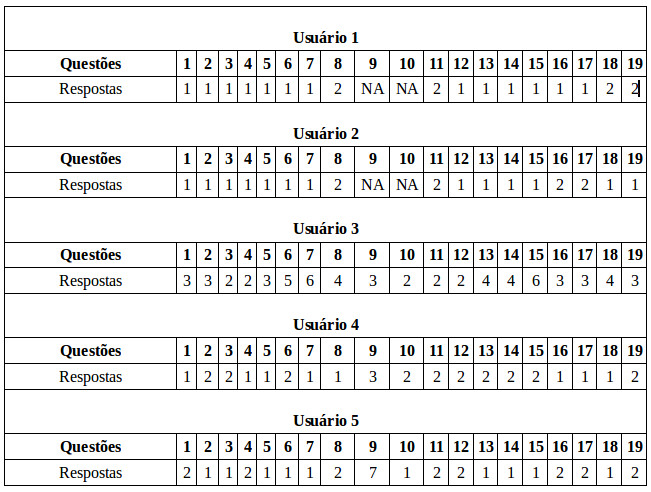
\includegraphics[scale=0.6]{figuras/pssuqalta_2.jpg}
  \caption{Resposta dos usuários ao questionário PSSUQ na segunda avaliação do protótipo de alta fidelidade}
  \label{pssuqalta_2}
  \end{figure}  
  
    \pagebreak
    \subsection{Análise dos resultados da avaliação do protótipo de alta fidelidade}
     
      
      \subsubsection{1ª iteração}
      
	Na primeira iteração o objetivo foi alcançado ao se obter um \textit{feedback} inicial da usabilidade do
	sistema, considerando as metas definidas. As violações heurísticas ocorridas foram tratadas e o protótipo foi
	incrementado para a próxima iteração de avaliação.
      
      \subsubsection{2ª iteração}
	
	Na segunda iteração, cujo objetivo ainda era avaliar os quesitos de usabilidade do protótipo, o objetivo também
	foi alcançado obtendo \textit{feedbacks} diferentes e pertinentes dos usuários. As violações heurísticas que surgiram
	foram analisadas e corridas, culminando na criação de outra versão do protótipo (V3.0, vide apêncice G).
	
	Por restrições 
	de tempo, não foi possível realizar outra iteração de avaliação com os usuários com a nova versão, ficando proposto apenas
	o planejamento da terceira iteração de avaliação.
      
      \subsubsection{Análise geral}
	
	As respostas oferecidas pelos usuários aos questionários ASQ e PSSUQ forneceram insumos para a análise da
	evolução do protótipo segundo os cenários de avaliação do protótipo e segundo a percepção do usuário.
	
	Lembrando que o padrão de resposta para os questionários ASQ e PSSUQ é um padrão gradativo de 7 escalas (de 1 a 7),
	onde quanto mais perto do 1, mais os usuários estão satisfeitos com as afirmações propostas. Essa informação é 
	bastante importante para a análise dos gráficos que serão apresentados abaixo. As informações de ambos os gráficos 
	estão relacionadas à percepção dos usuários em relação ao protótipo.\\
	
	\noindent
	\emph{\textbf{Análise dos cenários pelo questionário ASQ}}
	
	A média das respostas dos usuários ao questionário ASQ para cada cenário de avaliação foi calculada, por
	iteração de avaliação, e o resultado é apresentado na figura \ref{evolucao_prototipo_alta_fidelidade_ASQ}.
	
	\begin{figure}[!htpb]
	  \centering
	  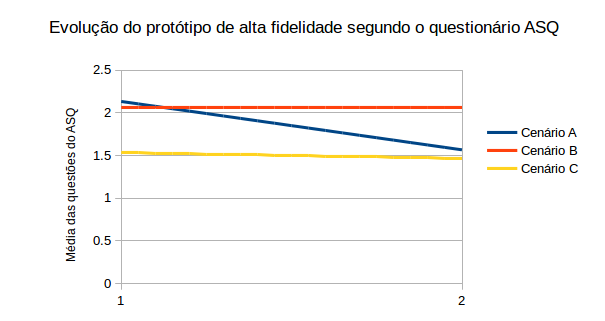
\includegraphics[scale=0.8]{editaveis/figuras/evolucao_prototipo_alta_fidelidade_ASQ}
	  \caption[Evolução dos cenários do protótipo de alta fidelidade, segundo o questionário ASQ]
	    {Evolução dos cenários do protótipo de alta fidelidade, segundo o questionário ASQ.}
	  \label{evolucao_prototipo_alta_fidelidade_ASQ}
	\end{figure}
	
	A partir do gráfico apresentado na figura \ref{evolucao_prototipo_alta_fidelidade_ASQ}, é possível observar que o 
	cenário A obteve uma evolução significativa da primeira iteração para a segunda iteração.
	O cenário B não apresentou mudanças significativas da primeira iteração para a segunda iteração. O cenário C apresentou 
	uma pequena evolução. Pela a análise dos cenários, é perceptível que os esforços pra incrementar o protótipo para uma 
	próxima iteração de avaliação devem se concentrar nos cenários B e C.\\
	
	\noindent
	\emph{\textbf{Análise da usabilidade pelas dimensões do PSSUQ}}
	
	A média das respostas dos usuários ao questionário PSSUQ para cada iteração de avaliação foi calculada e
	o resultado é apresentado na figura \ref{evolucao_prototipo_PSSUQ}.
	Foram avaliadas separadamente as quatro dimensões do PSSUQ para acompanhar a evolução de cada dimensão.
	
	\begin{figure}[!htpb]
	  \centering
	  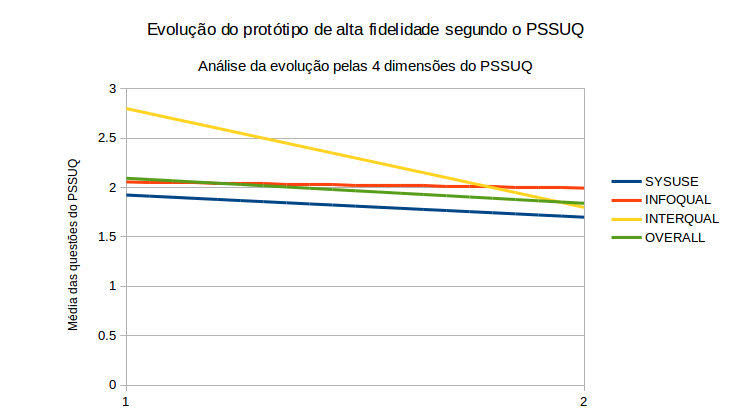
\includegraphics[scale=0.8]{editaveis/figuras/evolucao_prototipo_PSSUQ}
	  \caption[Evolução do protótipo de alta fidelidade, segundo as dimensões do questionário PSSUQ]
	    {Evolução do protótipo de alta fidelidade, segundo as dimensões do questionário PSSUQ.}
	  \label{evolucao_prototipo_PSSUQ}
	\end{figure}
	
	Pelo gráfico apresentado na figura \ref{evolucao_prototipo_PSSUQ} nota-se que ambas as dimensões obtiveram 
	evoluções, destacando-se as dimensões \textit{SysUse} e \textit{InterQual} que tiveram mudanças mais significativas, embora
	a dimensão \textit{SysUse} tenha apresentado um evolução não muito grande.
	A dimensão \textit{InfoQual} foi a que menos evoluiu da primeira iteração para a segunda iteração. Destaca-se, então,
	que os esforços de correções devem ser aplicados nos quesitos trazidos pelas dimensões \textit{SysUse} e \textit{InfoQual},
	mais relacionadas com as metas de eficácia e eficiência.
	
	A dimensão \textit{Overall} está relacionada com a percepção geral do protótipo e está intrisecamente relacionado com as 
	demais dimensões, não sendo possível evoluir sozinha. Por esse motivo, apresentou uma evolução ligeiramente razoável da primeira
	para a segunda iteração de avaliação.
      
      
    
